\chapter{Systematic Uncertainties}
\label{cha:SystematicUncertainties}

Since it is not always possible to determine the ideal set of values for a particular analytical technique, estimates of systematic errors are performed here.
This is done by making small variations to a particular value, while holding the rest constant, and looking at how the end results change.
14 sources of systematic errors are studied (labeled 0-13), the first 13 are given in table~\ref{tab:sysErrorSources} along with the number of variations and description for each source.
The 14th source of systematic error is variations in the 6 sectors of CLAS; a separate section below is dedicated to this topic.

\section{Sector Dependence}
\label{sec:SectorDependence}
In reality, the 6 sectors of CLAS are not identical.
To account for this, sector dependence is included in the systematic error studies.
As can be seen in figure~\ref{fig:sectorDep_0_1_4_3}, the variations are both statistical and systematic.
To avoid double counting the statistical error, the total error is assumed to be:
%
\begin{equation}
\label{eq:totalError_stat_sys}
\sigma^2 = \sigma^2_{stat} + \sigma^2_{sys}
\end{equation}
%
and the systematic error is then simply:
%
\begin{equation}
\label{eq:sysError_sectorDep}
\sigma^2_{sys} = \sigma^2 - \sigma^2_{stat}.
\end{equation}
%
In the rare cases when $\sigma^2_{stat}$ is larger than $\sigma^2$, the systematic error is taken to be zero.
%
\begin{figure}[htp]
\centering
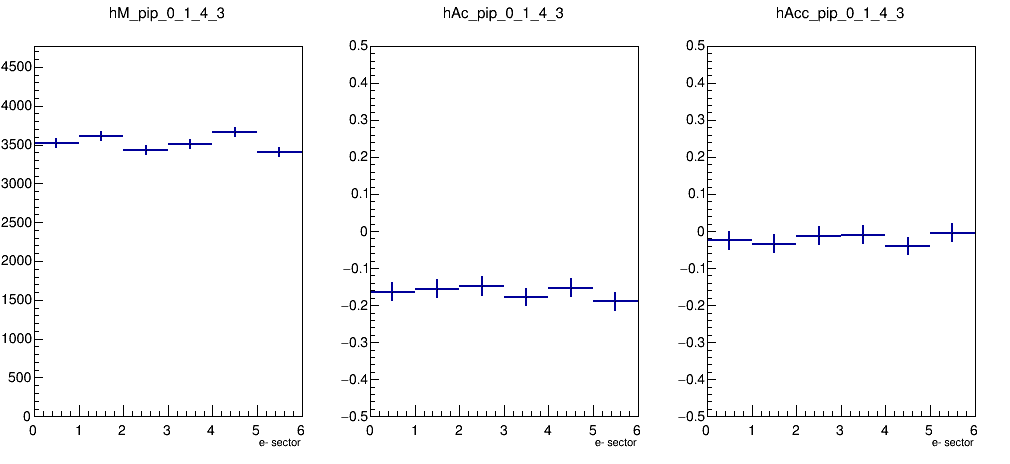
\includegraphics[width=6in]{figures/sectorDep_0_1_4_3.png}
\caption{Measurements of $A_0$, $A^{\cos\phi}$, and $A^{\cos2\phi}$ for a representitive bin as a function of the electron sector.}
\label{fig:sectorDep_0_1_4_3}
\end{figure}
%

\section{Other Sources of Systematic Uncertainty}
\label{sec:OtherSystematicUncertainty}
The systematic error on the final result due to a given source is the RMS of the deviations of the modified result from the original, i.e. the error from source $i$ is
%
\begin{equation}
\label{eq:RMS}
\Delta_{RMS}^i = \frac{\sqrt{\sum_j^{N_v^i} \Delta_j^2}}{\sqrt{N_v^i}}
\end{equation}
%
where $\Delta_j$ is the difference between the final result with the nominal value and the final result with variation $j$, and $N_v^i$ is the number of variations for source $i$.
``Final result'' refers to the values of $A_0$, $A_{UU}^{\cos\phi_h}$, and $A_{UU}^{\cos 2\phi_h}$ for each kinematic bin (systematic errors are calculated for each quantity).
The sources of systematic error are assumed to be uncorrelated and therefore are added in quadrature to get the total systematic error.
In the case of a cut value, there are two variations: a looser cut and a tighter cut.
In the case of model dependence, there is one variation: the second to last iteration.
%
\begin{table}[htp]
\centering
%\begin{tabular}{c l c l}
\begin{tabular}{ p{1.5cm} p{3cm} p{2cm} p{6cm} }
\hline
\textbf{Label} & \textbf{Source} & \textbf{\# of variations} & \textbf{Description}\\ \hline
0 & e- z-vertex cut & 2 & cut value is loosened or tightened by 0.2 cm on each side \\
1 & e- EC sampling cut & 2 & see figure~\ref{fig:eSystematicCuts} \\
2 & e- EC outer vs inner cut & 2 & cut value is loosened or tightened by 0.005 GeV \\
3 & e- EC geometric cut & 2 & see figure~\ref{fig:eSystematicCuts} \\
4 & e- CC $\theta$ matching cut & 2 & see figure~\ref{fig:eSystematicCuts} \\
5 & e- region 1 fiducial cut & 2 & see figure~\ref{fig:eSystematicCuts} \\
6 & e- region 3 fiducial cut & 2 & see figure~\ref{fig:eSystematicCuts} \\
7 & e- CC fiducial cut & 2 & see figure~\ref{fig:eSystematicCuts} \\
8 & pion $\beta$ cut & 2 & cut is loosened or tightened by $0.25\sigma$ on both the low and high side \\
9 & pion region 1 fiducial cut & 2 & see figure~\ref{fig:pionSystematicCuts} \\
10 & $\phi_h$ fiducial cut & 2 & a bin ($10^\circ$) on each side is added or removed \\
11 & acceptance model dependence & 1 & the second to last iteration is used \\
12 & radiative correction model dependence & 1 & the second to last iteration is used \\
\hline
\end{tabular}
\caption{13 of the 14 sources of systematic error studied. The other source is sector dependence, which is handled separately.}
\label{tab:sysErrorSources}
\end{table}
%
\begin{sidewaysfigure}[htp]
\centering
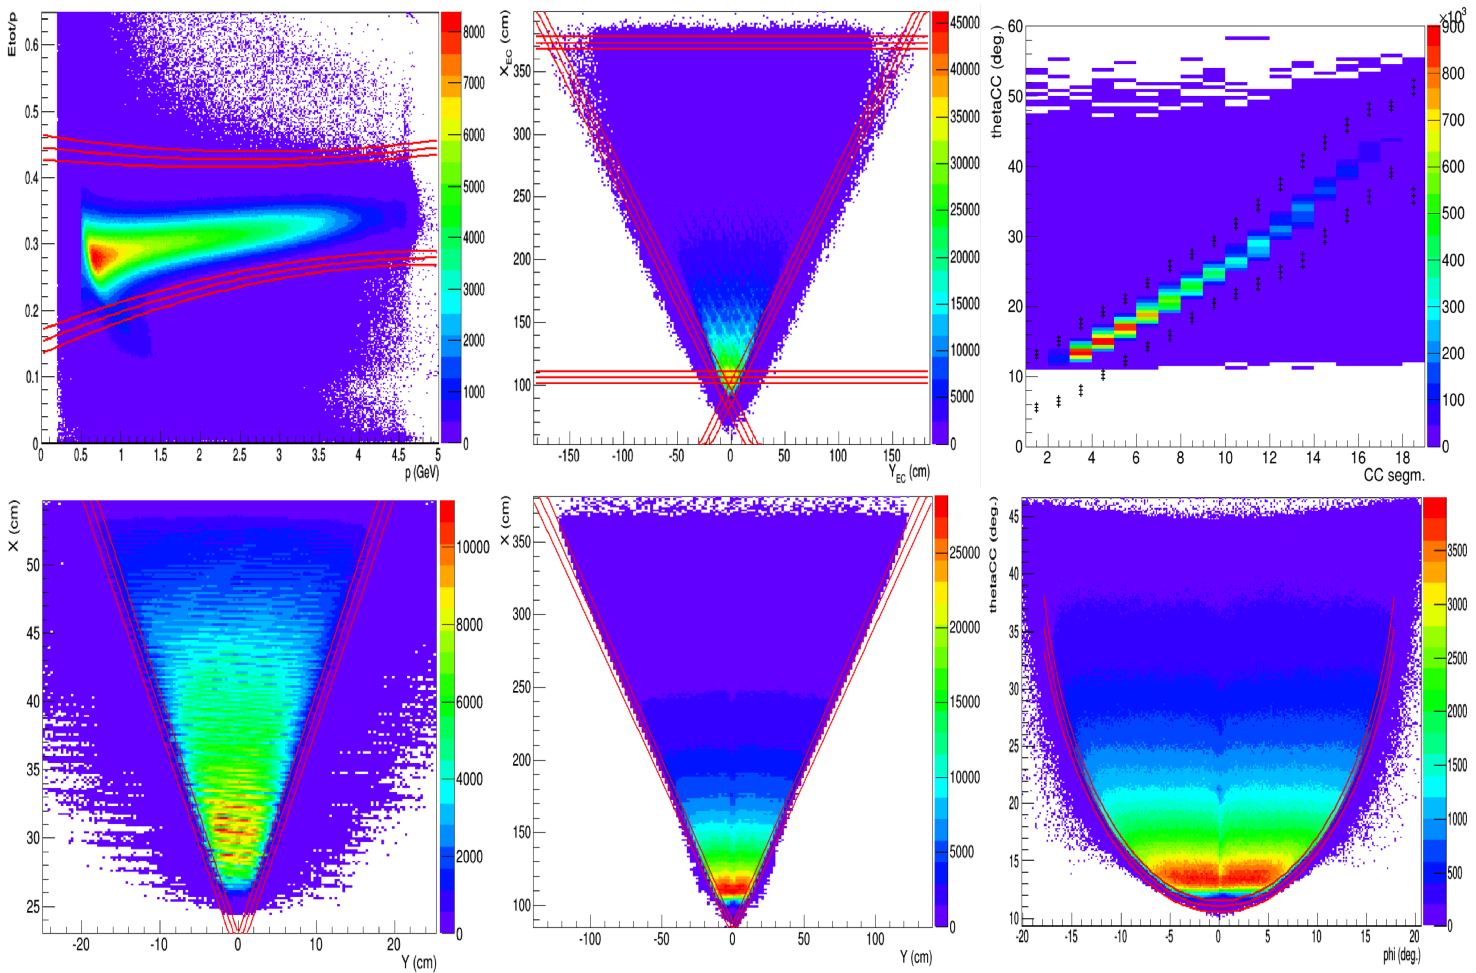
\includegraphics[width=8.5in]{figures/eSystematicCuts.png}
\caption{The loose, nominal, and tight cuts for six electron ID plots used for calculating systematic errors.}
\label{fig:eSystematicCuts}
\end{sidewaysfigure}
%
\begin{figure}[htp]
\centering
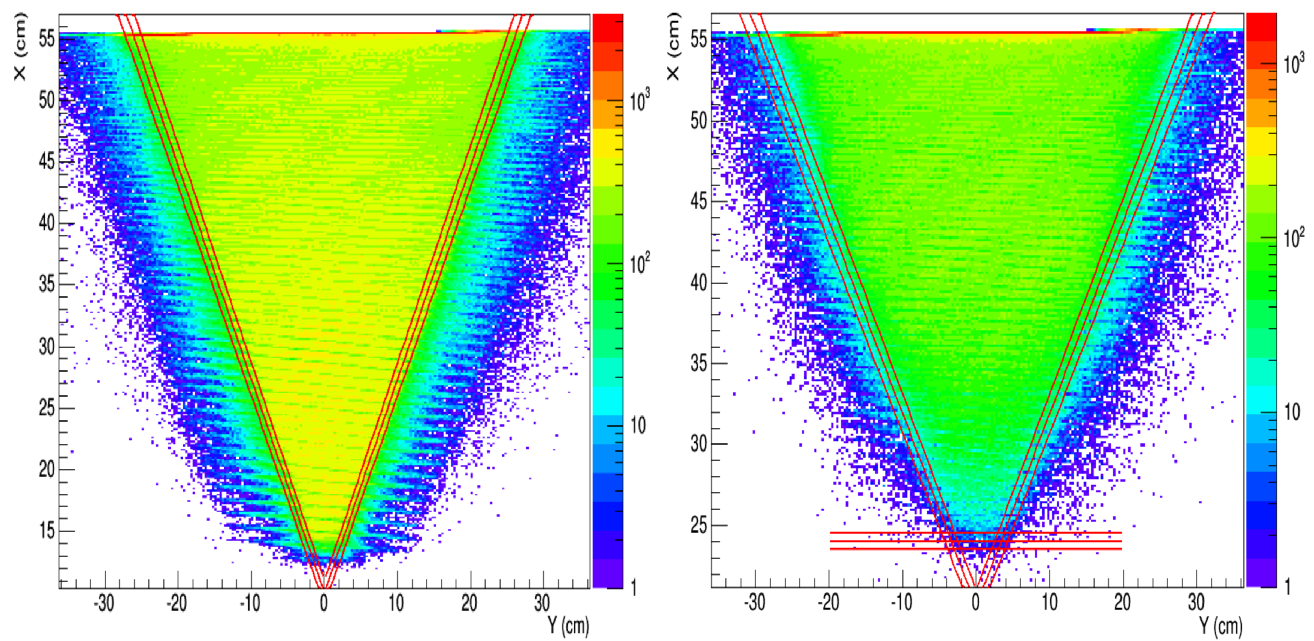
\includegraphics[width=6in]{figures/pionSystematicCuts.png}
\caption{The loose, nominal, and tight cuts for the region 1 fiducial cut for $\pi^+$ (left) and $\pi^-$ (right) used for calculating systematic errors.}
\label{fig:pionSystematicCuts}
\end{figure}
%
Figure~\ref{fig:systematicErrors_representitiveBin} shows the systematic error contribution of each source on $A_0$, $A_{UU}^{\cos\phi_h}$, and $A_{UU}^{\cos 2\phi_h}$ for a representitive bin.
%
\begin{figure}[htp]
\centering
%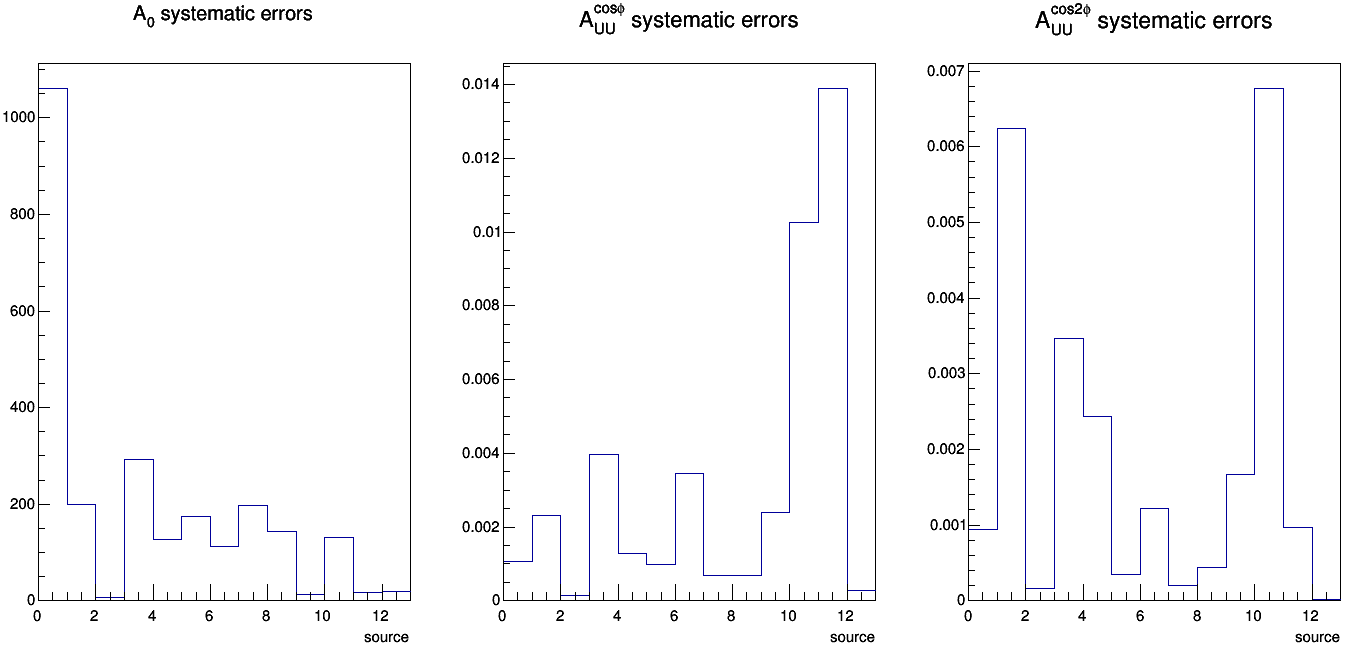
\includegraphics[width=6in]{figures/systematicErrors_representitiveBin.png}
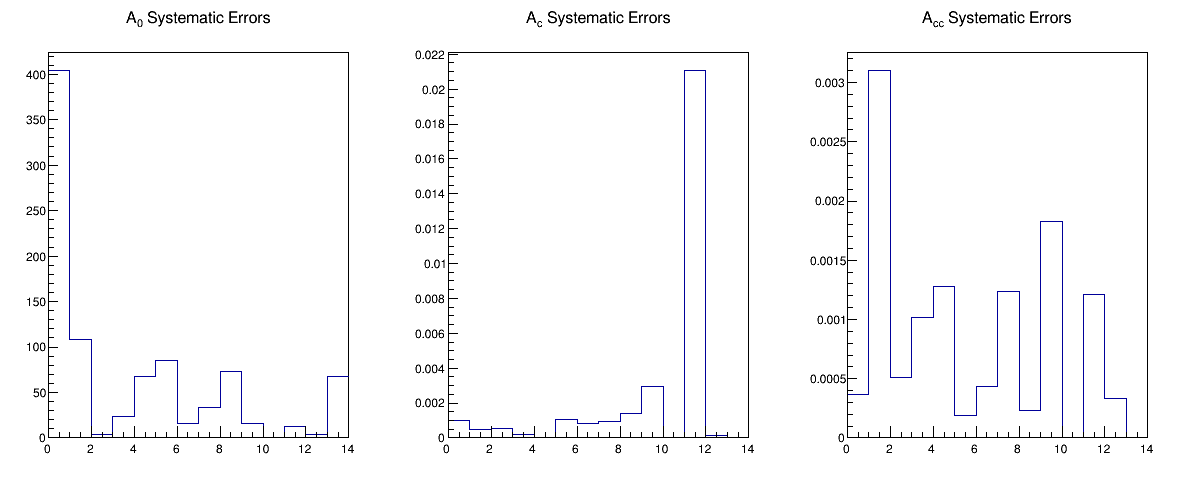
\includegraphics[width=6in]{figures/allSystematics_0_1_4_3.png}
\caption{Systematic errors on $A_0$, $A_{UU}^{\cos\phi_h}$, and $A_{UU}^{\cos 2\phi_h}$ for each source for a representitive bin.}
\label{fig:systematicErrors_representitiveBin}
\end{figure}
%

\clearpage
